% §IV --- Methodology (~2.25 pages, ~2000 words). Drafted D7.
% All formulas track ding/policy/ppo.py + ding/model/template/{vac.py,
% hppo_shared.py} bit-exactly.
\section{Methodology}\label{sec:method}

We now cast the problem in Section~\ref{sec:system} as a decentralized
partially observable Markov decision process and present \method, a
multi-agent hybrid PPO that learns over the resulting joint hybrid
action space. Section~\ref{subsec:dec-pomdp} formalizes the Dec-POMDP;
Section~\ref{subsec:problem} states the joint optimization problem;
Section~\ref{subsec:state} defines the state, action, and reward
structures; Section~\ref{subsec:mahppo} introduces
the actor / critic architecture with centralized training and
decentralized execution; Algorithm~\ref{alg:mahppo} summarizes the
training procedure.

\subsection{Dec-POMDP Formulation}\label{subsec:dec-pomdp}
We model the multi-UAV semantic offloading problem as a Dec-POMDP
$\langle\mathcal{U},\mathcal{S},\{\mathcal{O}_m\}_{m\in\mathcal{U}},
\{\mathcal{A}_m\}_{m\in\mathcal{U}},P,r,\gamma\rangle$. Agents are the
$M$ UAVs in $\mathcal{U}$; UEs are passive devices whose discrete and
continuous decisions (symbol cardinality, channel selector, transmit
power) are emitted by the joint policy alongside the per-UAV decisions.
The global state $s_t\in\mathcal{S}$ aggregates every device's position,
the per-channel SINR, the current channel-gain vector
$\boldsymbol{h}(t)$, the current symbol indices, the channel
assignment, and the normalized step index $t/T_s$. Each UAV agent
observes a local view $o_{m,t}\in\mathcal{O}_m$ that is identical to
$s_t$ in our centralized-execution implementation but is reserved as a
formal hook for future fully decentralized variants
(\S\ref{sec:limit}). The transition kernel $P(s_{t+1}\mid s_t,a_t)$ is
implicitly defined by the dynamics in
Sections~\ref{subsec:channel}--\ref{subsec:cost}. The discount factor
is $\gamma\in(0,1)$.

\subsection{Joint Optimization Problem}\label{subsec:problem}
Combining the joint system consumption metric of \eqref{eq:cost} with
the physical constraints derived in Section~\ref{sec:system}, we
formulate the slot-wise optimization problem as
\begin{subequations}\label{eq:problem}
\begin{align}
\min_{\mathbf{P},\mathbf{K},\mathbf{B},\mathbf{d},\boldsymbol{\theta}}
  \;\; & O(t) \\
\text{s.t.}\;\;
  & 0 \le p_{U,m}(t) \le P^{\max}_U,\quad m\in\mathcal{U}, \\
  & 0 \le p_{n}(t) \le P^{\max}_{n},\quad n\in\mathcal{N}, \\
  & K_{U,m}(t)\in\mathcal{K}_I,\;\; K_n(t)\in\mathcal{K}_T,\quad
    \forall m,n, \\
  & b_{i}(t)\in\mathcal{C},\quad i\in\mathcal{I},\\
  & B_{t,i} = B_c/n_{t,b_{i}(t)},\quad i\in\mathcal{I}, \\
  & 0 \le \Delta d_{m}(t) \le D_{\max},\quad m\in\mathcal{U}, \\
  & 0 \le \theta_{m}(t)\le \pi,\quad m\in\mathcal{U}, \\
  & \xi^{(\ell(n,t),n)}_{t}\ge \xi_{\mathrm{th}},\quad n\in\mathcal{N}.
\end{align}
\end{subequations}
Constraints (10b)--(10c) cap transmit powers; (10d) restricts symbol
cardinalities to predefined codebook sets $\mathcal{K}_I$ (UAV side)
and $\mathcal{K}_T$ (UE side); (10e)--(10f) implement orthogonal
co-channel sharing; (10g)--(10h) bound UAV per-slot displacement and
heading; (10i) enforces a minimum semantic similarity from the offline
DeepSC-VQA LUT, ensuring that any episode that ``succeeds'' actually
preserves task fidelity. The joint nature of \eqref{eq:problem} is what
prevents direct application of conventional convex optimization: the
LUT term $\xi^{(\ell(n,t),n)}_t$ depends on every other variable through
the SINR \eqref{eq:snr} and the closest-UAV association \eqref{eq:assoc}.

\subsection{State, Action, and Reward Spaces}\label{subsec:state}
\paragraph{State.} The global state at slot $t$ is
\begin{equation}
\begin{aligned}
s(t) = \big\{\,&d_{\mathrm{BS}},\,\{d_m(t)\}_{m\in\mathcal{U}},\,
              \{d_n(t)\}_{n\in\mathcal{N}},\\
              &\{\gamma_{t,i},h_{t,i},b_{t,i},K_{t,i}\}_{i\in\mathcal{I}},\,
              t/T_s\,\big\},
\end{aligned}
\label{eq:state}
\end{equation}
flattened to a vector of dimension $7(M+N)+4$. The dimension scales
linearly with the number of devices, which matches the architecture
described in Section~\ref{subsec:mahppo}.

\paragraph{Action.} The joint action factorizes into a discrete part and
a continuous part:
\begin{equation}
\begin{aligned}
a(t) = \big(\,&\underbrace{\{K_{U,m},b_{U,m}\}_{m=1}^{M}\cup
  \{K_{n},b_{n}\}_{n=1}^{N}}_{\text{discrete }a^{d}(t)},\\
  &\underbrace{\{\Delta d_{m},\theta_{m},p_{U,m}\}_{m=1}^{M}\cup
  \{p_{n}\}_{n=1}^{N}}_{\text{continuous }a^{c}(t)}\,\big).
\end{aligned}
\label{eq:action}
\end{equation}
This is a $2(M+N)$-head discrete action and a $(3M+N)$-dim continuous
action; the policy outputs them under the factorized hybrid
distribution
$\pi_{\theta}(a\mid s)=\pi_{\theta_d}^{d}(a^{d}\mid s)\,\pi_{\theta_c}^{c}(a^{c}\mid s)$.

\paragraph{Piecewise reward.} The reward at slot $t$ is the four-branch
piecewise function
\begin{equation}\small
r(t) =
\begin{cases}
+\eta_{\mathrm{succ}},
  & \mathcal{S}(t),\\[2pt]
-\eta_{\mathrm{fail}},
  & t>T_{\max},\\[2pt]
-\alpha_{1}O(t)+\alpha_{2}D(t)+\alpha_{3},
  & \neg\mathcal{S}(t)\wedge\mathcal{F}_{\xi}(t),\\[2pt]
-\alpha_{1}O(t)+\alpha_{2}D(t)-\alpha_{4}\rho_{\mathrm{sim}}(t),
  & \text{otherwise},
\end{cases}
\label{eq:reward}
\end{equation}
where $\mathcal{S}(t)\!\equiv\![O(t)\!<\!O^{*}\wedge\xi^{(\ell(n,t),n)}_{t}\!\ge\!\xi_{\mathrm{th}}\;\forall n]$
denotes a successful slot and $\mathcal{F}_{\xi}(t)\!\equiv\![\xi^{(\ell(n,t),n)}_{t}\!\ge\!\xi_{\mathrm{th}}\;\forall n]$
denotes a similarity-feasible slot.
$D(t)\in[0,1]$ is a normalized distance term that encourages
trajectory stability ($D(t)=1-\bar{d}_{U}(t)/R_{\mathrm{cell}}$ with
$\bar{d}_{U}$ the mean UAV-to-BS horizontal distance);
$\rho_{\mathrm{sim}}(t)$ is the fraction of UEs whose semantic
similarity falls below the threshold $\xi_{\mathrm{th}}$; $O^{*}$ is the
target consumption bound; $T_{\max}$ is the episode length cap; and
$(\eta_{\mathrm{succ}},\eta_{\mathrm{fail}},\alpha_{1\ldots4})$ are
hyperparameters listed in Table~\ref{tab:params}. Successful semantic
delivery yields $+\eta_{\mathrm{succ}}$, episode termination without
success yields $-\eta_{\mathrm{fail}}$; the third and fourth branches
provide dense gradient signal over the cost--similarity manifold so that
gradient flow remains informative even when neither terminal event has
fired. We additionally use a curriculum on the trade-off coefficient
$\alpha$ in \eqref{eq:cost}: $\alpha$ starts at $0$ (energy-only) for
the first $L_{1}$ training iterations and is linearly annealed to its
target value over the next $L_{2}$ iterations, mirroring the
schedule used in trust-region monotonic improvement work
\cite{schulman2015trpo,kuba2022happo}.

\subsection{\method: Multi-Agent HPPO with CTDE}\label{subsec:mahppo}
\method follows the centralized-training, decentralized-execution
paradigm \cite{lowe2017maddpg,yu2022mappo}. The actor and critic share a
trunk encoder $\phi_{\psi}(s_{t})\in\mathbb{R}^{H}$ realized as a
feed-forward MLP with width
$[265,128,128,64]$ and layer normalization. A centralized value head
$V_{\phi}(s_{t})$ outputs the global state value used to compute the
generalized advantage estimator
\cite{schulman2017ppo}.

The actor is split into a \emph{discrete branch} and a
\emph{continuous branch}. The discrete branch realizes the
$2(M+N)$-head joint distribution by stacking Dueling heads
\cite{wang2016dueling}: in the role-aware variant we use one
specialized $\mathrm{DuelingHead}_{i}$ per slot $i\in\{1,\dots,2(M+N)\}$
(this is the conference VAC behaviour preserved as the MA-HPPO main
result), while the parameter-shared MAPPO-hybrid baseline applies one
shared $\mathrm{DuelingHead}$ per role group $\{$UAV-symbol,
UE-symbol, UAV-channel, UE-channel$\}$ to a per-agent embedding
$\phi_{\psi}(s_{t})+e_{m}$ obtained by adding a learned index
embedding $e_{m}$. The continuous branch is a single
$\mathrm{Reparameterization}$ head producing a tanh-bounded Gaussian
$\mathcal{N}(\mu_{\theta_{c}}(s_{t}),\sigma^{2}\,\mathbf{I})$ over the
$(3M+N)$-dim continuous action; we use a fixed $\sigma=0.2$ in our
experiments to stabilize early-training exploration.

\begin{figure}[t]
  \centering
  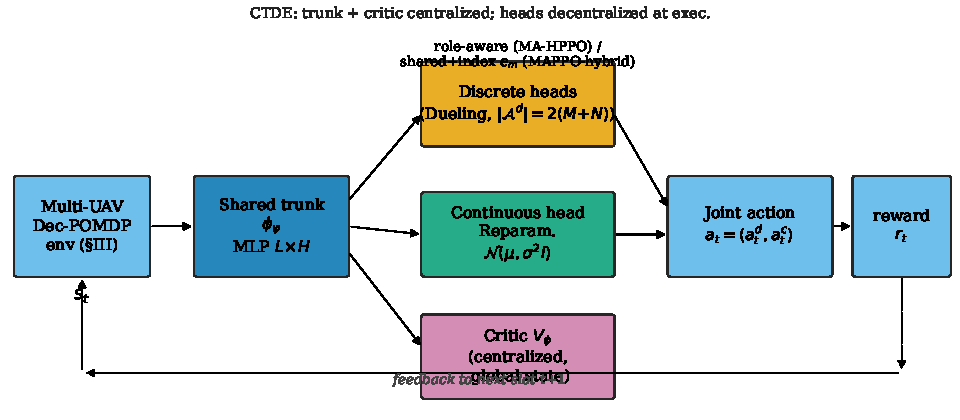
\includegraphics[width=0.95\linewidth]{figures/fig2_arch.pdf}
  \caption{\method architecture under centralized training and
  decentralized execution. The shared trunk encoder $\phi_{\psi}$
  consumes the global state and emits a per-agent embedding. The
  discrete branch uses one Dueling head per UAV / UE / channel slot in
  the role-aware MA-HPPO; the parameter-shared MAPPO-hybrid baseline
  shares one head per role group across agents via a learned index
  embedding $e_m$. The continuous branch produces a $(3M+N)$-dim
  Gaussian policy over per-UAV trajectory $(\Delta d, \theta)$ and
  per-device transmit power. The centralized critic outputs the global
  state value used by the GAE.}
  \label{fig:arch}
\end{figure}

The clipped surrogate objective is the sum of a discrete and a
continuous PPO loss with shared advantage $\hat{A}_{t}$ and value-loss
weights $w_{v}, w_{e}$:
\begin{align}
\mathcal{L}^{d}(\theta_{d})
  &= \mathbb{E}_{t}\!\Big[\min\!\big(r^{d}_{t}(\theta_{d})\hat{A}_{t},
        \mathrm{clip}\big(r^{d}_{t}(\theta_{d}),1-\epsilon,1+\epsilon\big)\hat{A}_{t}\big)\Big],
        \label{eq:lossd}\\
\mathcal{L}^{c}(\theta_{c})
  &= \mathbb{E}_{t}\!\Big[\min\!\big(r^{c}_{t}(\theta_{c})\hat{A}_{t},
        \mathrm{clip}\big(r^{c}_{t}(\theta_{c}),1-\epsilon,1+\epsilon\big)\hat{A}_{t}\big)\Big],
        \label{eq:lossc}\\
\mathcal{L}^{\mathrm{tot}}
  &= -\big(\mathcal{L}^{d}+\mathcal{L}^{c}\big)
     + w_{v}\,\mathbb{E}_{t}\!\big[(V_{\phi}(s_{t})-V^{\mathrm{tgt}}_{t})^{2}\big]
     - w_{e}\,\mathbb{E}_{t}\!\big[\mathcal{H}^{d}_{\theta_{d}}(s_{t})
       +\mathcal{H}^{c}_{\theta_{c}}(s_{t})\big],\label{eq:losstot}
\end{align}
where $r^{d}_{t}$ and $r^{c}_{t}$ are the per-factor importance ratios,
$V^{\mathrm{tgt}}_{t}$ is the GAE-bootstrapped target,
$\mathcal{H}^{d}$ and $\mathcal{H}^{c}$ are the discrete and continuous
policy entropies, and $\epsilon$ is the clip ratio. The factorized
hybrid policy admits an additive policy gradient that we develop
formally in Section~\ref{sec:theory}; here we note only that
\eqref{eq:lossd}--\eqref{eq:losstot} reduce to standard discrete and
continuous PPO when one of the two action sides is empty.

\subsection{Training Procedure}\label{subsec:train}
\method is on-policy. Each iteration collects $n_{\mathrm{sample}}$
transitions across $E_{\mathrm{coll}}$ parallel environments, computes
GAE advantages with $(\gamma,\lambda)$, and performs $K_{\mathrm{epoch}}$
mini-batch updates of $\mathcal{L}^{\mathrm{tot}}$. Algorithm
\ref{alg:mahppo} summarizes the procedure; Table~\ref{tab:params}
reports the hyperparameter values used in
Section~\ref{sec:exp}.

\begin{algorithm}[t]
  \caption{\method-Based Joint Resource Allocation for Multi-UAV
  Semantic Communication}
  \label{alg:mahppo}
  \begin{algorithmic}[1]
    \REQUIRE Encoder $\phi_{\psi}$, actor $(\theta_{d},\theta_{c})$,
             critic $\phi$; clip $\epsilon$, weights $w_{v},w_{e}$;
             discount $\gamma$, GAE $\lambda$; mini-batch size $B$;
             epochs $K_{\mathrm{epoch}}$; rollout $n_{\mathrm{sample}}$.
    \ENSURE Trained parameters $(\psi,\theta_{d},\theta_{c},\phi)$.
    \STATE Initialize $(\psi,\theta_{d},\theta_{c},\phi)$ and the
           replay buffer $\mathcal{D}\leftarrow\emptyset$.
    \STATE Set old policies $\theta^{\mathrm{old}}\leftarrow\theta$.
    \FOR{iteration $\ell=1,2,\dots,L$}
      \STATE Reset all environments and obtain $s_{0}$.
      \FOR{$t=0,\dots,n_{\mathrm{sample}}-1$}
        \STATE Sample $a^{d}_{t}\sim\pi^{d}_{\theta^{\mathrm{old}}_{d}}(\cdot\mid s_{t})$,
               $a^{c}_{t}\sim\pi^{c}_{\theta^{\mathrm{old}}_{c}}(\cdot\mid s_{t})$.
        \STATE Form $a_{t}=(a^{d}_{t},a^{c}_{t})$, execute, observe
               $r_{t},s_{t+1}$; store $(s_{t},a_{t},r_{t},s_{t+1})$ in
               $\mathcal{D}$.
      \ENDFOR
      \STATE Compute GAE advantages $\hat{A}_{t}$ and value targets
             $V^{\mathrm{tgt}}_{t}$ using $V_{\phi}$ over $\mathcal{D}$.
      \STATE Normalize $\hat{A}_{t}$ within the batch.
      \FOR{epoch $k=1,\dots,K_{\mathrm{epoch}}$}
        \FOR{mini-batch $\mathcal{B}\subset\mathcal{D},\;|\mathcal{B}|=B$}
          \STATE Compute $\mathcal{L}^{d},\mathcal{L}^{c}$ via
                 \eqref{eq:lossd}--\eqref{eq:lossc} on $\mathcal{B}$.
          \STATE Compute $\mathcal{L}^{\mathrm{tot}}$ via
                 \eqref{eq:losstot} on $\mathcal{B}$.
          \STATE Update $(\psi,\theta_{d},\theta_{c},\phi)\leftarrow$
                 Adam-step on $\nabla\mathcal{L}^{\mathrm{tot}}$.
        \ENDFOR
      \ENDFOR
      \STATE $\theta^{\mathrm{old}}\leftarrow\theta$;
             clear $\mathcal{D}$.
    \ENDFOR
  \end{algorithmic}
\end{algorithm}
